This section surveys related studies first. 
Following this, a new hybrid morphological tagging algorithm is described detailing its components and architecture. 
Finally, the presented tool is evaluated through several experiments showing its high performance.

\subsection{Background}

First of all, we overview how morphological tagger systems are typically built up. 
Since there are just a few tools performing the full task, we also review \gls{pos} tagging attempts for morphologically rich languages. 
In addition, previous approaches for Hungarian are introduced as well. %, hence Hungarian plays an important role in our experiments.

\subsubsection{Full morphological tagging}

There has been insufficient discussion about full morphological tagging in recent studies of natural language technology. 
The reason behind this is that most of the attempts concentrate on morphologically not very rich languages (such as English), where \gls{pos} tagging is generally sufficient, and the ambiguity of the lemmatization task is negligible. 
Furthermore, there are studies (following English approaches) which ignore lemmatization (such as~\cite{Hajic1998a,Tufis1998,Silfverberg2011}) even for highly inflectional languages. 

Nevertheless, approaches on full morphological tagging can be grouped depending on their relationship to lemmatization.

\begin{enumerate}
  \item First of all, numerous researchers propose a two stage model, where the first phase is responsible for finding full morpho-syntactic tags, while the second one is for identifying lemmata for \emph{(word, tag)} pairs. 
  For instance, Erjavec and Dzeroski decompose the problem~\cite{Erjavec2004} by utilizing a trigram  tagger first, then applying a decision list lemmatizer. \label{part:general-lemmatization}
  Further on, Agič et al. combine~\cite{Agic2013} an \acrshort{hmm}-based tagger with a data-driven rule-based lemmatizer~\cite{Jongejan}. 
  Even though such combinations could have error propagation issues, they usually result in well-established accuracy.
  \item Another feasible approach is to treat the tagging task as a disambiguation problem. 
  Such methods utilize morphological analyzers to generate annotations candidates, then employ disambiguation methods for selecting correct analyses.
  These architectures are typical e.g. for Turkish attempts (cf.~\cite{Sak2007,Hakkani-Tur2002}).
  %, but similar studies are also published for Czech (such as~\cite{valamelyikHajic}) as well. 
  A drawback of this approach is that the disambiguation component depends heavily on the language-dependent analyzer used.
  \item Finally, the problem can be handled as a unified tagging task.
  An example is the Morfette system~\cite{Chrupaa2008}.
  It employs a joint architecture for tagging words both with their tags and lemmata considering lemmatization as a labeling problem.
  The tool represents a lemma class as a transformation sequence describing string modifications from the surface form to the root.
  Further on, Morfette utilizes the \acrshort{maxent} framework and employs separate models for each of the subtasks yet using a joint beam search decoder.
  Another similar method was presented by Laki and Orosz~\cite{Laki2013} recently.
  Their system (HuLaPos) merges \gls{pos} labels with lemmata transformation sequences to a unified tag, which is then learned by the Moses statistical machine translation framework \cite{Koehn2007}.
  Therefore, HuLaPos can translate sentences to sequences of labels.
  These joint approaches are usually language independent, however, they can either be slow to train or inaccurate due to the increased search space they use.
\end{enumerate}

Considering lemmatization (case \ref{part:general-lemmatization} above), the task can be easily accomplished by utilizing linguistic rules or lemma dictionaries. 
However, the creation of such resources is time-consuming.
Next, a general baseline method is to select the most frequent lemmata for each \emph{(word, tag)} relying on the training data (as in~\cite{zsibrata2013magyarlanc}). 
Despite its simplicity, this method usually results in mediocre precision systems.
Further on, employing advanced \gls{ml} algorithms is also a viable approach.
E.g. Plisson et al. apply ripple down rule induction algorithms~\cite{Plisson2004} for learning suffix transformations.
Even though they report about good results, their attempt ignores the dependency between tags and lemmata.
Next, Jongejan and Dalianis generate decision lists (cf. CST method~\cite{Jongejan}) for handling morphological changes in affixes.
However, their system is optimized for inflecting languages exploring complex changes in word forms.  

\subsubsection{Morpho-syntactic tagging of morphologically rich languages}

Next we describe how well-known data-driven \gls{pos} tagging methods are applied for morphologically rich languages focusing on issues yielded by the complexity of the morphology.
In doing so, only data-driven models are reviewed investigating techniques for managing
\begin{enumerate}
  \item the increased number of out-of-vocabulary word forms and
  \item the large complexity of the tag-set. 
\end{enumerate}

While numerous attempts have been published for tagging Polish recently~\cite{Piasecki2006,Piasecki2007,Acedanski2010,Radziszewski2013},  performance of these tools are below the average.
Most of these solutions (e.g. \cite{Radziszewski2013}) use morphological analyzers to get morpho-syntactic tag candidates to reduce the search space of the decoder used.
Further on, tiered tagging is another widely utilized technique~\cite{Radziszewski2013}.
This method resolves complex tags by computing its parts one after another.
Considering \acrshort{ml} algorithms used, the range of applications is wide.
Beside an adaptation of Brill’s tagger~\cite{Acedanski2010}, C4.5 decision trees~\cite{Piasecki2007}, memory-based learning~\cite{Radziszewski2011} and \acrshort{crf} models are employed~\cite{Radziszewski2013} as well. 

Moving on, the first successful attempt to analyze Czech was published by Hajič and Hladká~\cite{Hajic1998a} basing on a discriminative model.
Their approach uses a morphological analyzer and builds on individual prediction models for ambiguity classes.
Actually, the best results for Czech are obtained using the combination of numerous systems~\cite{Hajic2007}.
In their solution, three different data-driven taggers (\acrshort{hmm}, \acrlong{maxent} and averaged perceptron) and further symbolic components are utilized as well.
A \acrshort{ma} computes the possible analyses, while the rule-based disambiguator tool removes agrammatical tag sequences. 

The flexible architecture of the Stanford tagger \cite{Toutanova2003} also allows the integration of various morphological features thus enabling its usage for morphologically rich languages.
An example is the Bulgarian tool~\cite{Georgiev2012} (by Georgiev et al.), which uses a morphological lexicon and an extended feature set.
Further on, applications of trigram tagging methods \cite{Brants2000,Halacsy2007} have been demonstrated (for example Croatian~\cite{Agic2013}, Slovenian~\cite{Agic2013} and Icelandic~\cite{Loftsson2007}) to be effective as well.
%In contrast with former studies, 
These systems achieve high accuracy utilizing large morphological lexicons and decent unknown word guessing algorithms.

Considering agglutinative languages, the usage of finite-state methods is indispensable for handling the huge number of possible wordforms.
E.g. Silferberg and Lindén introduce a trigram tagger for Finnish~\cite{Silfverberg2011} that is based on a weighted finite-state model.
As regards Turkish, Daybelge and Cicelki describe a system~\cite{Daybelge2007} employing also a finite-state rule-based method.
However, most taggers for agglutinative languages use hybrid architectures incorporating morphological analyzers into stochastic learning methods.
Examples are the perceptron-based application of Sak et al.~\cite{Sak2007} and the trigram tagging approach of Dilek et al.~\cite{Hakkani-Tur2002}.

Recent approaches include the results of the Statistical Parsing of Morphologically Rich Languages workshop \cite{SPMRL:2010,SPMRL:2011,SPMRL:2012,SPMRL:2013}.
First, Le Roux et al. \cite{leroux2012} presented an accurate parser for Spanish relying on the morphological annotations of Morfette \cite{Chrupaa2008}.
Further on, Bengoetxea et al. \cite{bengoetxea2011testing} showed that tagging quality greatly influences the accuracy of parsing Basque. 
For this, they used a tagger based on \acrlong{hmm}s combined with a symbolic component.
Next, Maier et al. \cite{maier2014} investigated the effect of the tag-set granularity on processing German. 
They concluded, that \acrshort{pos} tagging can be performed more accurately using less granular tags, while both the coarse-grained and too fine-grained morpho-syntactic labels decrease the parsing performance.

Most recently, Bohnet et al. have introduced methods \cite{bohnet2013joint} for the joint morphological and syntactic analysis  of richly inflected languages.
Their best solutions involve the usage of morphological analyzers and word clusters, resulting in significant improvements on parsing of all the tested languages.
However, their method requires syntactically annotated texts restricting the applicability of the algorithm for less-resourced domains.
Further on, Müller et al. \cite{mueller2013} improved on \acrshort{crf}-based methods to apply them effectively on the morpho-syntactic tagging of morphologically rich languages.
The proposed system uses a coarse-to-fine mapping on tags for speeding-up the training of the underlying discriminative method.
In this way, their solution can go beyond general 1\textsuperscript{st}-order models thus resulting in increased accuracy.
Their best systems utilize complex morpho-syntactic features and outputs of morphological analyzers as well.

To summarize, effective methods for morphologically complex languages rely on either a discriminative or a generative model.
Such taggers generally use morphological lexicons or analyzers to handle the large vocabulary of the target language.
Further on, tagging of unknown words is a crucial problem being managed by either guessing modules or rich morphological features. 

\subsubsection{The case of Hungarian}

As regards Hungarian \gls{pos} tagging, the first attempt was performed by Megyesi~\cite{Megyesi1998} adapting Brill’s transformation-based method~\cite{Brill1992}. 
Since she did not use any morphological lexicon, her approach resulted in moderate success.
Similarly, Horváth et al. investigated \cite{Horvath1999} only pure machine learning algorithms (such as C4.5 or instance based learning) resulting in low accuracy systems.
Three years later, the first promising approach was presented by Oravecz and Dienes~\cite{Oravecz2002a} utilizing TnT~\cite{Brants2000} with a weighted finite-state lexical model.
In 2006, Halácsy et al. investigated an augmented \acrshort{maxent} model~\cite{Halacsy2006} in combination with language specific morphological features and a \acrshort{ma}.
In that study, the best result was achieved by combining the latter model with a trigram-based tagger.
Later, they created the HunPos system~\cite{Halacsy2007}, which reimplements and extends TnT.
Their results (with a morphological lexicon) has been shown to be as efficient as the one of Oravecz and Dienes~\cite{Oravecz2002a}.
Next, Kuba et al. applied boosting and bagging techniques for transformation based learning \cite{Kuba2004}.
Although they managed to reduce the error rate of the baseline tagger, their results lag behind previous approaches.
Recently, Zsibrita et al. published \texttt{magyarlanc}~\cite{zsibrata2013magyarlanc}, a natural language processing chain specially designed for Hungarian.
They adapted the Stanford tagger \cite{Toutanova2003} in two steps. 
First, to train the underlying discriminative method effectively, a tag-transformation step is applied reducing the number of morpho-syntactic labels.
Next, the tool utilizes a morphological analyzer as well to enhance and speed up the disambiguation process.

Most of the previous approaches concentrated on the morpho-syntactic tagging task, thus there are only three tools which performs lemmatization as well and can be applied to Hungarian.
\begin{enumerate}
	\item \texttt{magyarlanc}, which builds on a \acrshort{maxent} model and employs a rule-based lemma guesser system.
	\item HuLaPos, which applies machine translation methods for the tagging task. 
	\item Morfette, which uses two \acrlong{maxent} models for jointly decoding both the labels and lemmata.
\end{enumerate}
Although, \texttt{magyarlanc} provides accurate annotations, the tool has two weaknesses which inhibit its applications on corpora having different annotation schemata. 
It does not provide a straightforward way to train and contains built-in annotation-specific components.
Further on, machine learning algorithms behind HuLaPos and Morfette need a large amount of training data to produce high accuracy, therefore it can be troublesome to apply them on less-resourced domains.
Finally, none of these tools contain components which would allow them to be adjusted for new domains without retraining them.

This chapter introduces a new morphological tagging tool, which uses simple trigram methods and employs a pluggable morphological analyzer component.
It differs from existing approaches in having a language and tag-set independent architecture yet producing high accuracy and also being flexible enough to be used in rule-based domain-adaptation scenarios.
PurePos is designed to operate on morphologically rich languages and resource-scarce scenarios, providing accurate annotations even when a limited amount of training data is available only.
Furthermore, our approach is shown to have very high accuracy on general Hungarian. %, while also having a short training time.

\subsection{The full morphological tagging model}
\label{sec:purepos}

The architecture of PurePos (cf. Figure \ref{fig:purepos-arch}) is composed of multiple components. 
The data flow starts from a \gls{ma} providing word analyses as \emph{(lemma, tag)} pairs. 
Next, a trigram model is used to select morpho-syntactic labels for words. 
Then, lemmatization is carried out using both statistical and linguistic components. 

\begin{figure}[H]
  \centering
  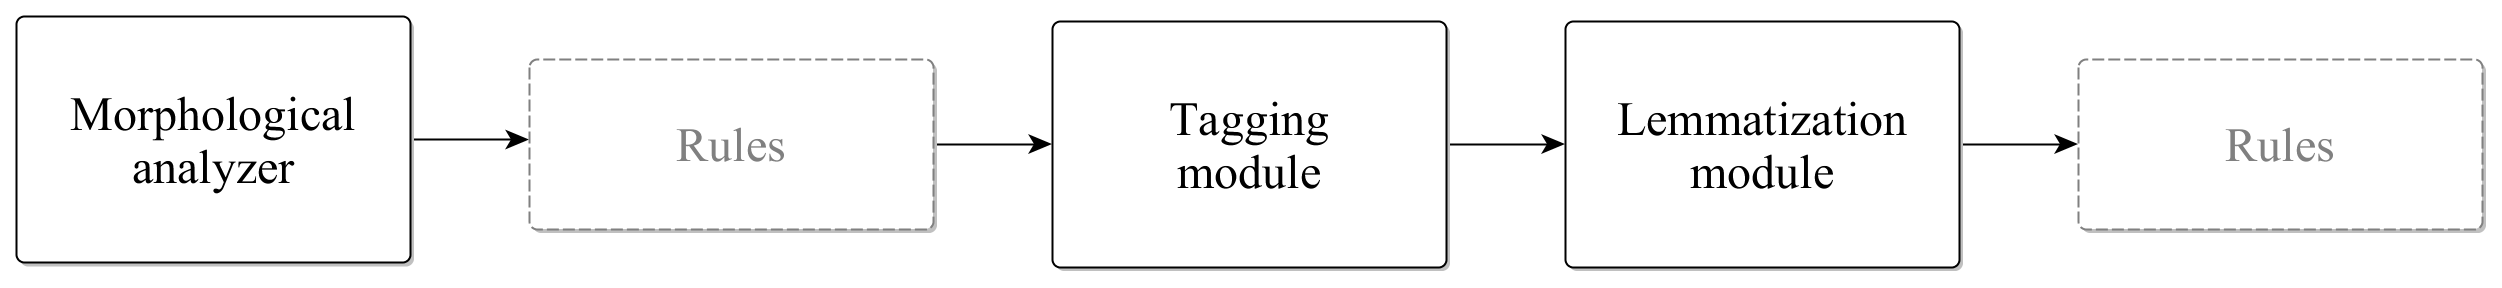
\includegraphics[width=1\textwidth]{MorphTagging/architecture.png} 
  \caption{The architecture of the proposed method}
  \label{fig:purepos-arch}
\end{figure}

In the following, we present its components making the morphological tagging effective. 
Underlying statistical models are introduced first, then we show how symbolic algorithms are incorporated. 

\subsubsection{The PoS tagging model}

\begin{figure}[H]
  \centering
  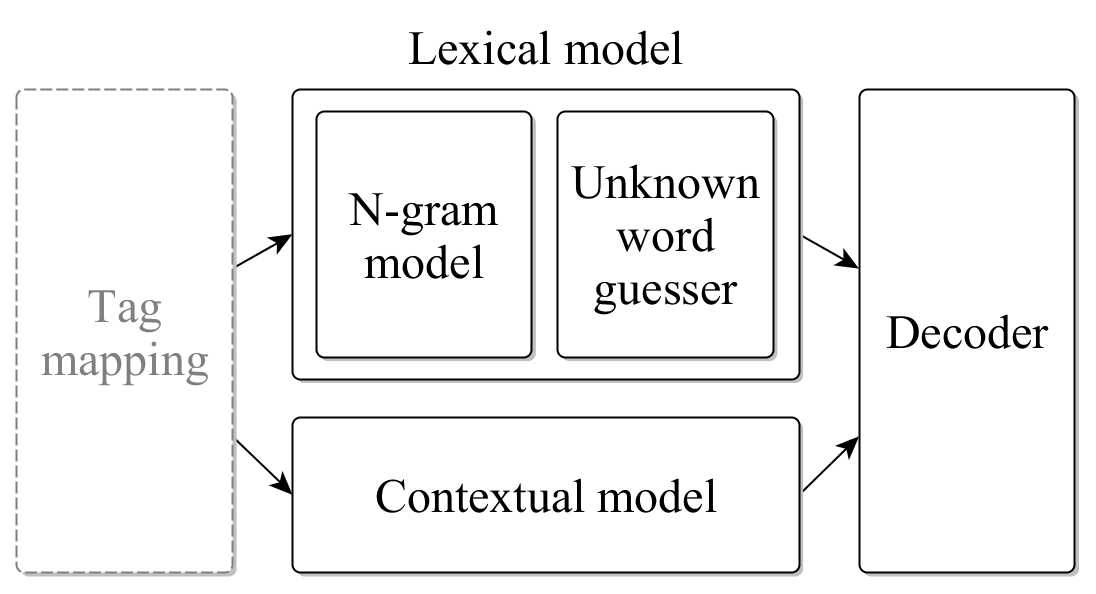
\includegraphics[width=0.5\textwidth]{MorphTagging/pos_arch.png} 
  \caption{Part-of-speech tagging in the proposed system}
  \label{fig:pos_arch}
\end{figure}

PurePos builds on \acrshort{hmm}-based methods \cite{Rabiner1989,Samuelsson1993} introduced in TnT \cite{Brants2000} and HunPos \cite{Halacsy2007}, allowing it to be fast, simple and effective at the same time. 
Our implementation (similarly to HunPos) allows the user to set the tagging order individually for both the contextual ($n_1$) and lexical model ($n_2$).
The method presented (see Figure \ref{fig:pos_arch}) selects the best fitting $t_1^m$ morpho-syntactic label sequence for the $m$ long $w_1^m$ sentence using individual contextual and lexical probabilities of tags and words (in the $i$th position):
\begin{equation}
\argmax_{t_1^m} \prod_{i=1}^m P(t_i | t_{i-1}^{i-n_1}) P(w_i|t_{i-1}^{i-n_2})
\end{equation}

Its contextual model is computed with simple $n$-gram language-modeling techniques (cf. Equation \ref{eq:purepos-contextual}) employing \gls{mle} (see Equations \ref{eq:purepos-contextual2a} and \ref{eq:purepos-contextual2b})\footnote{Where $N$ denotes the size of the tag-set, while $c(x)$ marks the number of $x$ elements in the training data.}. 
Uni-, bi- and trigram estimates are combined with deleted interpolation thus calculating $\lambda_k$ weights as suggested by Brants \cite{Brants2000}. Even though the order of the model is usually set to 3, it is adjustable in practice. 


\begin{equation}\label{eq:purepos-contextual}
P(t_i | t_{i-1}^{i-n_1}) \approx \sum_{k=0}^{n_1-1} \lambda_k \hat{P}(t_i|t_{i-1}^{i-k})
\end{equation}

\begin{equation}\label{eq:purepos-contextual2a}
\hat{P}(t_i|t_{i-1}^{i-k}) = \frac{c(t^{i-k}_i)}{c(t_{i-1}^{i-k})} (k>0) 
\end{equation}
\begin{equation}\label{eq:purepos-contextual2b}
\hat{P}(t_i) = \frac{c(t_i)}{N} (k=0)
\end{equation}

Next, the lexical model ($P(w_i|t_{i-1}^{i-n_2}$) of our method is composed of two components. 
The first one handles tokens previously seen in the training data, while the second guesses labels for unknown words. 
In fact, each subsystem is doubled (as it is in \cite{Brants2000,Halacsy2007}) maintaining separate models for uppercase and lowercase words. 

Handling of previously seen words is carried out approximating $P(w_i | t_{i}^{i-n_2})$ with word-tag co-occurrences: 
\begin{equation} \label{eq:purepos-lexical}
P(w_i | t_{i}^{i-n_2}) \approx  \sum_{k=0}^{n_2-1} \lambda_k \hat{P}(w_i|t_{i}^{i-k})
\end{equation}

\label{sec:purepos-guesser}
$\hat{P}(w_i|t_{i}^{i-k})$ is calculated with \acrlong{mle}, while deleted interpolation is applied with $\lambda_k$ weights. 
As in the contextual model, $k$ is set to 2 in applications.

As regards tagging of unknown words, we use -- in accordance with Brants -- the distribution of rare\footnote{Rare words are considered to be those that occur less than 10 times in the training data.}
tokens’ tags for estimating their \gls{pos} label. 
Since suffixes are strong predictors for tags in agglutinative languages, we use the last $l$ letters ($\{s_{n-l+1} \dots s_n\}$) for estimating probabilities. 
Successive abstraction is utilized in our tool as described in \cite{Samuelsson1993,Brants2000}.
This method calculates the probability of a $t$ tag recursively using suffixes with decreasing lengths: 

\begin{align}
 P(t|s_{n-l+1}, \dots, l_n) 
 \approx \frac{ \hat{P}(t|s_{n-l+1}, \dots, s_n) + \theta \hat{P}(t|s_{n-l}, \dots, s_n)}{1+\theta}
\end{align}

$\theta$ parameters are computed utilizing the standard deviation of the maximum likelihood probabilities of all the $k$ tags:

\begin{align}
	\theta = \frac{1}{k-1}\sum_{j=1}^k(\hat{P}(t_j)-\overline{P})^2
\end{align}

where

\begin{align}
	\overline{P} = \frac{1}{k}\sum_{j=1}^{k}\hat{P}(t_j)
\end{align}

Finally, \gls{mle} is employed for calculating both $\hat{P}(t_j)$ and $\hat{P}(t|s_{n-l+1}, \dots, s_n)$. 


Concerning decoding, beam search is utilized, since it can yield multiple tagging sequences at the same time. 
In that way, the tool is also able to produce tagging scores of sentences \eqref{eq:purepos-score} allowing us to incorporate further components using partly disambiguated word sequences. 

\begin{equation}\label{eq:purepos-score} %%TODO: ez történik, kell ez ide?
Score(w_1^m,t_1^m) = \log \prod_{i=1}^m P(w_i|t_i,t_{i-1})P(t_i|t_{i-1},t_{i-2})P(l_i|t_i,w_i)
\end{equation}

\subsubsection{The lemmatization model}

\begin{figure}[H]
  \centering
  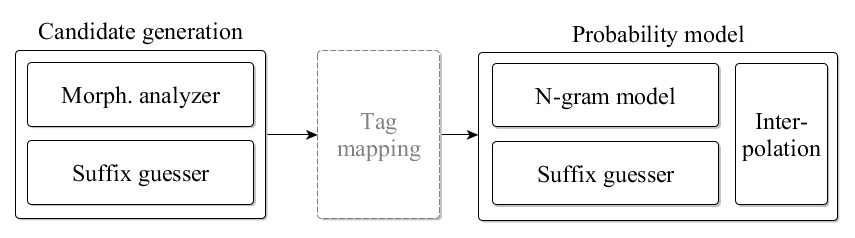
\includegraphics[width=0.8\textwidth]{MorphTagging/lemma_arch.png} 
  \caption{The data flow in the lemmatization component}
  \label{fig:lemma-arch}
\end{figure}

Lemmatization is performed in two steps (cf. Figure \ref{fig:lemma-arch}). 
First, candidates are generated for \emph{(word, morpho-syntactic tag)} pairs. 
If morphological analyses are available for the current word, their lemmata are used as candidates, otherwise suffix-based guessing is carried out. 
For this, the guesser (described in Section \ref{sec:purepos-guesser}) was extended to handle lemma transformations as well. 
Combined labels can represent both the morpho-syntactic tag and suffix-transformations for lemmata (for an example see Table \ref{tab:lemma-example}).


\begin{table}[H]
\centering
\caption{Examples for the combined representation of the tag and lemma}
\label{tab:lemma-example}
\begin{tabular}{l | l l}
   \textbf{Word} &  \emph{házam} `my houses’ &  \emph{baglyot} `owl’ \\
   \textbf{Tag} &  \textsc{n.1}s\textsc{pos} &  \textsc{n.acc} \\
   \textbf{Lemma} &  \emph{ház} `house’ &  \emph{bagoly} `owl’ \\
   \textbf{Transformation} & -2+$\varnothing$ &  -4+\emph{oly} \\
   \textbf{Combined label} & (\textsc{n.1}s\textsc{pos}, -2,--) &  (\textsc{n.acc}, -4, \emph{oly}) \\
\end{tabular}
\end{table}


As for picking the right lemma, we utilize a simple scoring model \eqref{lemma-max} that evaluates candidates using their part-of-speech tags:
\begin{equation}\label{lemma-max}
\argmax_l S(l|t,w)
\end{equation}
This method is based on a twofold estimation of $P(l|t,w)$. On the one hand, a unigram lemma model ($P(l)$) calculates conditional probabilities using relative frequency estimates. 
On the other hand, reformulation of $P(l|t,w)$ yields another approximation method:
\begin{equation}\label{lemma-guesser}
P(l|t,w) = \frac{P(l,t|w)}{P(t|w)}
\end{equation}

Substituting this formula to \eqref{lemma-max}, $P(t|w)$ becomes a constant which can be omitted. 
In that way, we can estimate $P(l,t|w)$ employing only the lemma guesser. 
Finally, models are aggregated in a unified ($S$) score: 
\begin{equation}\label{lemma-interpolated}
S(l|w,t) = P(l)^{\lambda_1} P(l,t|w)^{\lambda_2}
\end{equation}


\begin{algorithm*}
\setstretch{1.35}
\begin{algorithmic}[H]
    \ForAll{(word, tag, lemma)} 
        \State candidates $\gets$ generateLemmaCandidates(word, tag)
        \State maxUnigramProb $\gets$ getMaxProb(candidates, word, tag, unigramModel)
        \State maxSuffixProb $\gets$ getMaxProb(candidates, word, tag, suffixModel)
        \State actUnigramProb $\gets$ getProb(word, tag, lemma, unigramModel)
        \State actSuffixProb $\gets$ getProb(word, tag, lemma, suffixModel)
        \State unigramProbDistance $\gets$ maxUnigramProb $-$ actUnigramProb
        \State suffixProbDistance $\gets$ maxSuffixProb $-$ actSuffixProb
        \If {unigramProbDistance $>$ suffixProbDistance}
            \State $\lambda_{2} \gets$ $\lambda_{2}$ $+$ unigramProbDistance $-$ suffixProbDistance
        \Else%If{unigramProbDistance $<$ suffixProbDistance}
            \State $\lambda_{1} \gets$ $\lambda_{1}$ $+$ suffixProbDistance $-$ unigramProbDistance
        \EndIf
    \EndFor
    \State normalize$( \lambda_{1}, \lambda_{2} )$
  \end{algorithmic}
  \caption{Calculating parameters of the lemmatization model}
\label{lemma-interpolation-algorithm}
\end{algorithm*}

The idea of computing $\lambda_{1,2}$ parameters is similar to that seen for the \gls{pos} $n$-gram models. 
However, instead of using positive weights, negative scores are stored for the better model.  
$\lambda_{k}$ is calculated iterating over words of the training data (cf. Algorithm \ref{lemma-interpolation-algorithm}):
\begin{enumerate}
  \item first, both components return the best roots for each \emph{(word, tag)} pair, 
  \item then probability estimates for the gold standard lemma are computed,
  \item next, (absolute) error rates of the models are calculated ,
  \item finally, the best model’s weight is decreased\footnote{Since probability estimates are between 0 and 1, decreasing a weight gives higher values.}.
\end{enumerate}
After these steps, $\lambda_k$ parameters are normalized.


\subsubsection{Hybridization}

Although, the framework proposed builds on an existing \gls{pos} tagging algorithm, it is extended with a new lemmatization model and is modified to fit agglutinative languages such as Hungarian. 
Hybridization steps listed below show the differences between PurePos and its predecessors \cite{Brants2000,Halacsy2007}.

\begin{description}
  \item[Morphological analyzer] \hfill \\
  First of all, a morphological analyzer is utilized throughout the whole process, therefore probability estimation is performed for valid\footnote{Valid analyses for a word are those which are proposed by the MA.} analyses only.
  \item[Linguistic rules] \hfill \\
  Next, the presented architecture allows rule-based components to modify the analyses of the \acrshort{ma}, in that way, bad candidates can be filtered out. Furthermore, lexical probability scores of analyses can be also given to PurePos, which are then used as context-dependent local distribution functions. 
  \item[Unseen tags] \hfill \\ 
  In contrast to TnT or HunPos, our system is able to handle unseen tags\footnote{Morpho-syntactic labels which are not seen in the training data.} properly. On the one hand, if a token has only one analysis not seen before, that one gets selected with 1 lexical probability. Further on, estimation of forthcoming tags is performed using a lower level (unigram) model in this case. On the other hand, the system can also calculate lexical and contextual scores for any tag previously not seen. This can be performed mapping latter tags to known ones using regular expressions.\footnote{For a complete example see Section \ref{sec:oldhungarian}.}
  \item[$k$-best output] \hfill \\
  Finally, our method decodes tags using beam search. One can generate partly disambiguated sentences being apt for linguistic post-processing. Further on, this facility allows the usage of advanced machine learning techniques resulting in more accurate parsing algorithms.
\end{description}


\subsection{Experiments}

\subsubsection{Tagging general Hungarian}\label{sec:porepos-gen}

First, PurePos is evaluated on Hungarian texts. 
We used the Szeged Corpus~\cite{Csendes2004} (SZC) for our experiments, since it is the only Hungarian resource which is manually annotated and is freely available. 
It contains general texts from six genres being annotated with detailed (MSD) morpho-syntactic tags~\cite{Erjavec2012} and lemmata. 

On the one hand, we used the original corpus (version 2.3\footnote{The \acrshort{ma} that provides MSD annotations is only compatible with this corpus variation.}).
On the other hand, a variant of the SZC was employed as well that is tagged with the analyses of Humor ~\cite{Proszeky1994,Novak2003,Proszeky2005}.
Using both of them, we could evaluate our algorithm with two different morphological annotation schemata.
They were split in 8:2 ratio (randomly) for training and testing (as in Table \ref{tab:szeged-corpus}) purposes. 
Since the two corpora are not aligned which each other (the transcribed one contains fewer sentences), results obtained on the two datasets are not directly comparable.


\begin{table}[H]
\centering
\caption{Dimensions of the corpora used}
\begin{tabular}{l r r r r}
  \hline
  & \multicolumn{2}{c}{MSD tag-set} & \multicolumn{2}{c}{Humor tag-set} \\
  &  Training set &  Test set &  Training set &  Test set  \\
  \hline
  Tokens &  1,232,384 &  254,880 &  980,225 &  214,123 \\
  Sentences &  68,321 &  13,778 &  56,792 &  14,198 \\
  Distinct tags &  1,032 &  716 &  983 &  656 \\
  \hline
\end{tabular}
\label{tab:szeged-corpus}
\end{table}

As a morphological analyzer is an integral part of our method, we tested the tool with two different modules. 
The first setting utilized the MSD tagged corpus and an analyzer extracted from \texttt{magyarlanc}, while the second one applied Humor on the transcribed corpus.

Evaluation was carried out measuring the overall accuracy of full annotations (i.e \emph{(morpho-syntactic tag, lemma)} pairs). 
For significance tests, we used the Wilcoxon matched-pairs signed-rank test at the 95\% confidence level dividing the test set into 100 data pairs.
Sentence-based accuracies were also provided in some cases. 
The latter metric was computed by considering a sentence to be correct only when all of its tokens are properly tagged. 

We compared our results with other morphological tagging tools available for Hungarian\footnote{Since, our aim was only to compare available tagger methods, not to optimize each of them, external tools were employed with their default settings.}. 
Firstly, taggers providing full morphological annotations such as \texttt{magyarlanc}, HuLaPos and Morfette\footnote{Version 3.5 is used.} were evaluated.  
Secondly, we assembled full morphological taggers from available components\footnote{\acrshort{pos} taggers are trained using the full morpho-syntactic labels of words.}, since two-phase architectures were also shown to be prosperous (e.g.~\cite{Agic2013,Erjavec2004}). 

Concerning \gls{pos} tagging, we used three of the most popular algorithms as baselines. These are the following:
\begin{itemize}
  \item the trigram tagging method of HunPos,
  \item averaged perceptron learning and
  \item the maximum entropy framework of the OpenNLP~\cite{Baldridge2002} toolkit.
\end{itemize}

As regards lemmatization, CST~\cite{Jongejan} and a simple baseline method (BL) were employed. 
The latter one assigns the most frequent lemmata to a previously seen \emph{(word, tag)} pairs, otherwise the root is considered to be the word itself.

Beside these components, tag dictionaries were prepared for HunPos, since it can employ such resources.  
At this point we simulated a setting, where the tagger was only loaded once.
Therefore, a large lexicon was prepared for the tool.
In that way, analyses of the 100,000 most frequent words of Hungarian were provided to the tagger\footnote{Frequencies are calculated relying on the results of the Szószablya project~\cite{Halacsy2004}.}.



\begin{table}[H]
 \centering
 \caption{Tagging accuracies of Hungarian taggers on the Szeged Corpus (annotated with MSD labels)}
\begin{tabular}{l r r r}
  \hline
   & \multirow{2}{*}{PoS tagging} & \multicolumn{2}{c}{Morph. tagging} \\
   & &  Token &  Sentence \\
  \hline
  \texttt{magyarlanc} &  96.50\% &  95.72\% &  54.52\% \\
  Morfette &  96.94\% &  92.24\% &  38.18\% \\
  HuLaPos &  96.90\% &   95.61\% & 54.57\% \\
  PurePos &  \underline{96.99\%} &  \underline{96.27\%} &  \underline{58.06\%} \\
  HunPos + BL &  96.71\% &  92.65\% &  36.06\% \\
  HunPos + CST &  96.71\% &  91.19\% &  35.31\% \\
  Maxent + BL &  95.63\% &  92.21\% &  34.82\% \\
  Maxent + CST &  95.63\% &  90.14\% &  29.70\% \\
  Perceptron + BL &  95.19\% &  91.16\% &  29.42\% \\
  Perceptron + CST &  95.19\% &  89.78\% &  27.91\% \\
  \hline
\end{tabular}
\label{tab:morphtag-orig}
\end{table}


\begin{table}[H]
 \centering
 \caption{Tagging accuracies of Hungarian taggers on the transcribed Szeged Corpus (annotated with Humor labels)}
\begin{tabular}{l r r r}
  \hline
   & \multirow{2}{*}{PoS tagging} & \multicolumn{2}{c}{Morph. tagging} \\
   & &  Token &  Sentence \\
  \hline
  Morfette &  97.60\% &  94.73\% &  51.58\% \\
  HuLaPos &  97.19\% &  95.53\% &   57.55\% \\
  PurePos &  \underline{98.65\%} &  \underline{98.58\%} &  \underline{81.78\%} \\
  HunPos + BL &  97.41\% &  89.93\% &  32.07\% \\
  HunPos + CST &  97.41\% &  94.69\% &  52.40\% \\
  Maxent + BL &  94.81\% &  88.82\% &  28.19\% \\
  Maxent + CST &  94.81\% &  92.33\% &  40.10\% \\
  Perceptron + BL &  95.97\% &  88.85\% &  29.11\% \\
  Perceptron + CST &  95.97\% &  93.32\% &  45.13\% \\
  \hline
\end{tabular}
\label{tab:morphtag-humor}
\end{table}

% % % % % % % % % % % % % % % % % % % % % % % % % % % % % % % % % % % %
First of all, there are notable discrepancies between the results on the two datasets (cf. Tables \ref{tab:morphtag-orig} and \ref{tab:morphtag-humor}). 
On the one hand, performance discrepancies can be explained by the morphological analyzers used.
These tools have different coverage, thus they affect the results of parsing chains built on them.
On the other hand, the two corpora utilize different annotation schemes:
\begin{itemize}
  \item First, the original corpus contains foreign and misspelled words being tagged with a uniform \textsc{x} tag. 
  Due to the various syntactic behavior of such tokens, their labels could not be estimated using their context or their suffix properly.
  \item Further on, date expressions and several named entities are tagged with a single MSD code resulting in lemmata composed of more than one words. (An example is \emph{Golden Eye-oztunk} `we visited the Golden Eye’ being lemmatized as \emph{Golden Eye-ozik} `to visit the Golden Eye’.) 
  Such phenomena could be hard to handle for lemmatizers.
\end{itemize}
These variations can have a huge impact on morphological disambiguation algorithms.
In our case, they decrease the accuracy of MSD-based systems, while allow Humor-based ones to produce better annotation  (since the corresponding corpus is free of such phenomena).

In general, results show that the best-performing systems are PurePos, HuLapos, \texttt{magyarlanc} and Morfette.
Besides, HunPos also achieves high \acrshort{pos} tagging scores, while the other two-stage taggers are far behind state-of-the-art results. 
As regards learning methods of the OpenNLP toolkit, their performance indicate that they cannot handle such labeling problems precisely.
Further on, both of the standalone lemmatizers degrade accuracy. 
This reduced performance can be due to their design: the baseline method was not prepared for handling unknown words, while CST was originally created for inflectional languages. 
An interesting difference between lemmatization scores is that the baseline (BL) strategy performs better on the original corpus, while the CST tool gives higher accuracy on the Humor-labeled dataset. 
A reason behind this phenomena can be that the latter dataset has higher lemma ambiguity (cf. Section \ref{par:lemma-ambiguity}) thus requiring advanced methods.

An explanation for the high morpho-syntactic labeling score of PurePos is that it uses morphological analyzers to get analysis candidates. 
This component can reduce the number of unknown words, thus enabling the system to provide better annotations.
While HunPos also uses such resources, it can only handle static lexicons, which limits its accuracy.
%In that way, the huge number of inflected word-forms could be handled accurately.

As regards \texttt{magyarlanc}, it also yields first-class results (95.72\% accuracy) on the MSD-tagged corpus.
However, its built-in language (and annotation scheme) specific components inhibited its application on the other corpus. 
Further on, HuLaPos is an interesting outlier.
It is based on pure stochastic methods, but it can still achieve high precision. 
These results can be explained by the larger contexts used by the underlying machine translation framework.
Next, Morfette also provides accurate annotations (concerning \acrshort{pos} labels only), however, it has problems with computing the roots of words.

Results show that PurePos provides the most accurate annotations amongst tested tools.
Further on, its advance over other systems is statistically significant (Wilcoxon test of paired samples, p < 0.05)\footnote{Pairwise tests were carried out comparing token-level accuracies of PurePos and other competing tools on each corpus.}.
In addition, sentence-based accuracies (especially on the Humor-tagged corpus) also confirms the superior performance of our method. 
These values reveal that most of the tools result in erroneously tagged sentences in more than half of the cases, while the same number for our method is much less (18\% on the transcribed corpus and 42\% on the original one). 

It was shown that the presented algorithm can produce high quality morpho-syntactic annotations handling the huge number of inflected forms of Hungarian.
Further on, it can also produce precise root candidates for both previously seen and unseen tokens due to its improved lemma computing method.
In that way, PurePos is a suitable tool for morphological tagging of Hungarian.
%
%Next, comparison of full annotation scores reveals that our lemmatization algorithm significantly outperforms others. 
%Furthermore, its lemmatization method outperforms all other systems available for Hungarian.

\subsubsection{Resource-scarce settings}

Next, PurePos is compared to other taggers on less-resourced scenarios.
For this, we use systems\footnote{Unfortunately, we could not measure the performance of \texttt{magyarlanc}, since the current release of the tool cannot be trained.}  and corpora described in Section \ref{sec:porepos-gen}.
To simulate such settings, when just a limited amount of training data is available, we trained all the taggers using a few thousand sentences only (cf. Table \ref{tab:small-szeged}).
As an evaluation, learning curves of systems are drawn on both versions of the test set.

\begin{table}[H]
\centering
\caption{The number of tokens and sentences used for training the taggers for simulating resource-scarce settings}
\label{tab:small-szeged}
\begin{tabular}{ r | r r r r r}
Sentences & 2,000 & 4,000 & 6,000 & 8,000 & 10,000 \\
Tokens (MSD-tagged corpus) & 13,555 & 26,496 & 53,563 & 79,916 & 107,113 \\
Tokens (Humor-tagged corpus) & 20,863 & 41,740 & 82, 964 & 121,026 & 146,816 \\
\end{tabular}
\end{table}


\begin{figure}[H]
  \centering
  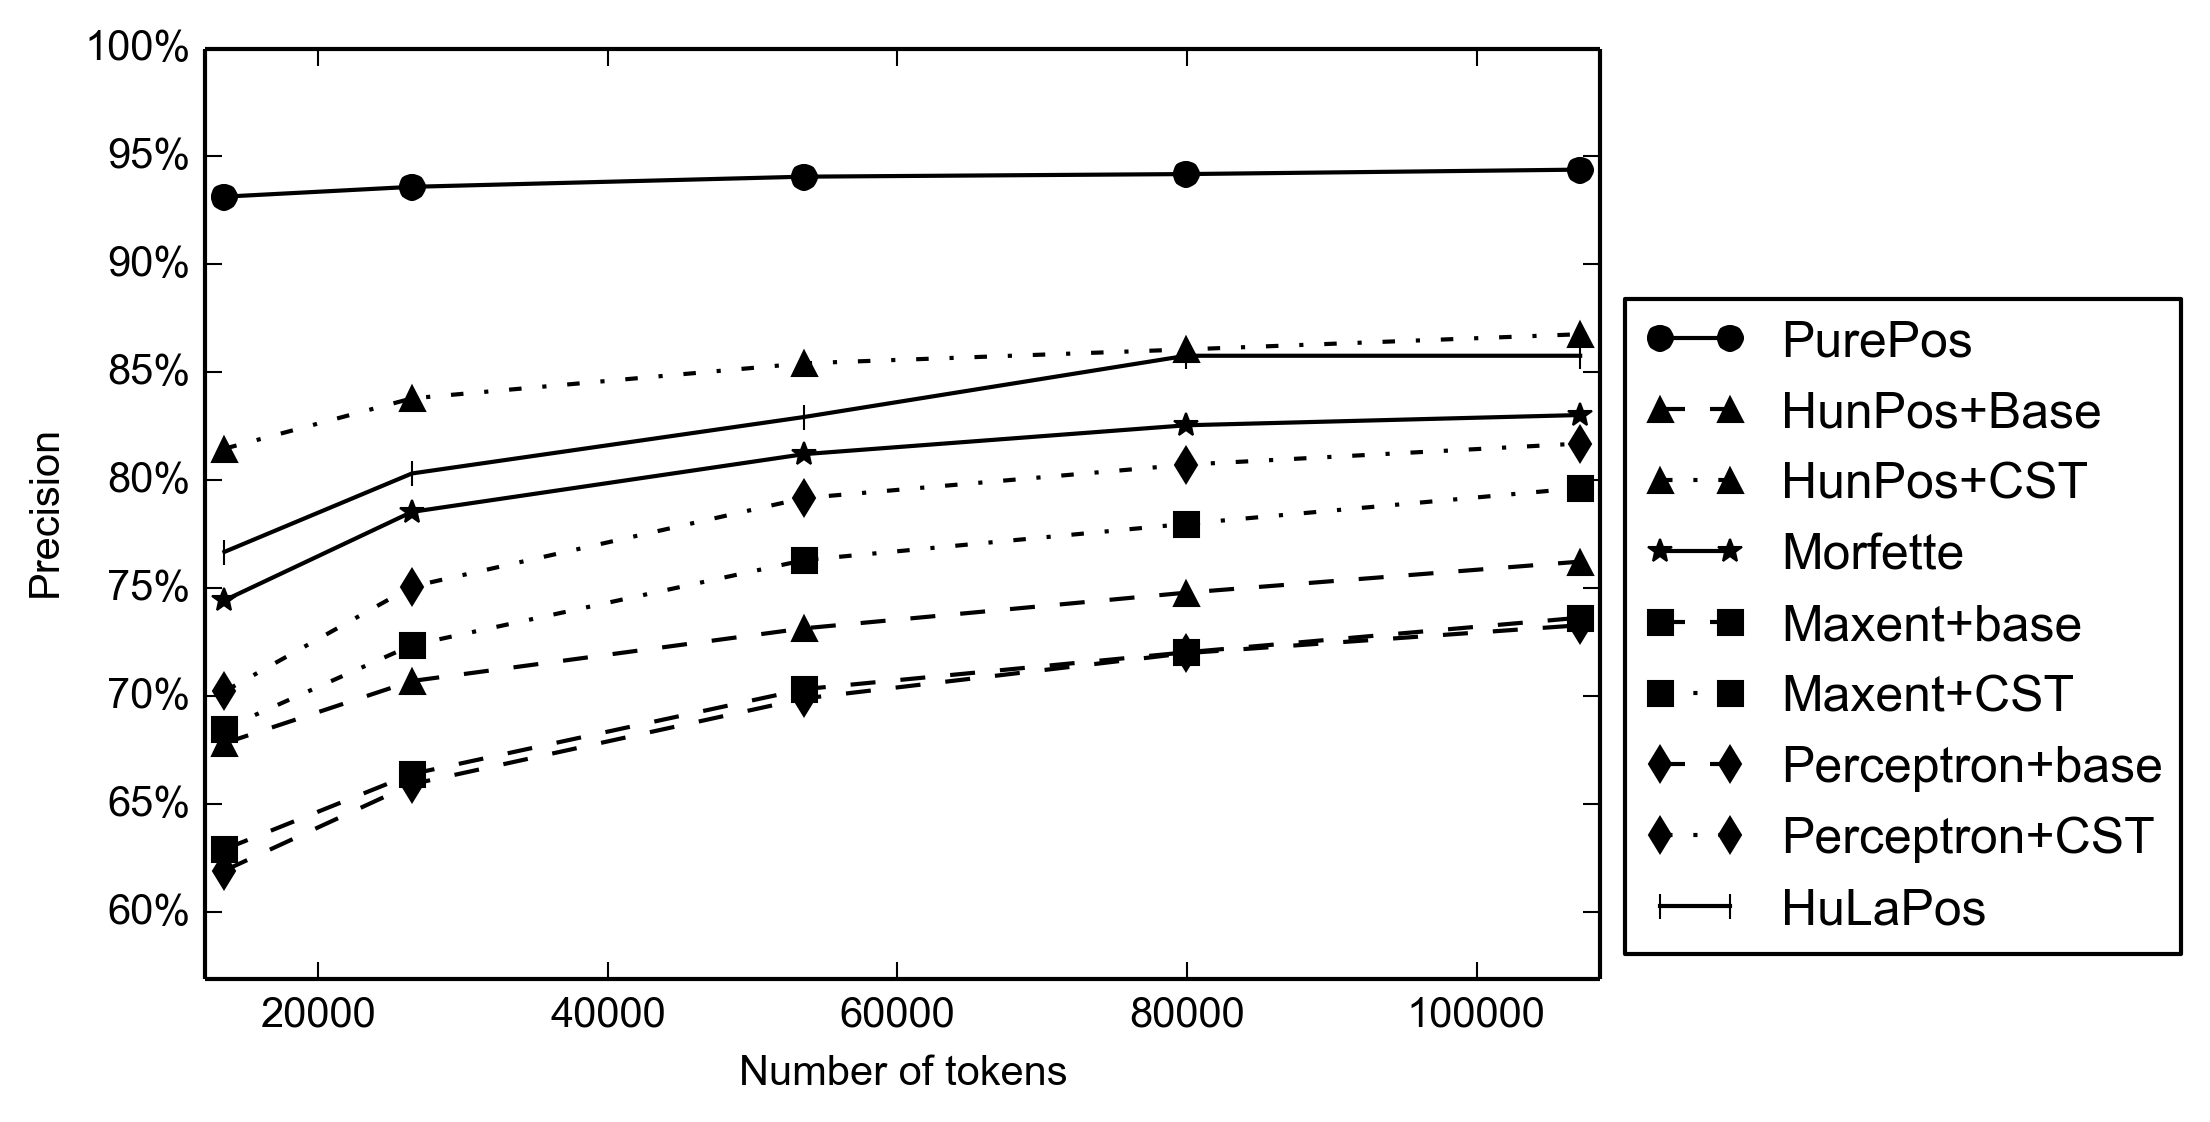
\includegraphics[width=1\textwidth]{MorphTagging/msd_token.png} 
  \caption{Learning curves (regarding token accuracy) of full morphological taggers on the Szeged Corpus (using MSD labels)}
  \label{fig:msd-token}
\end{figure}

\begin{figure}[H]
  \centering
  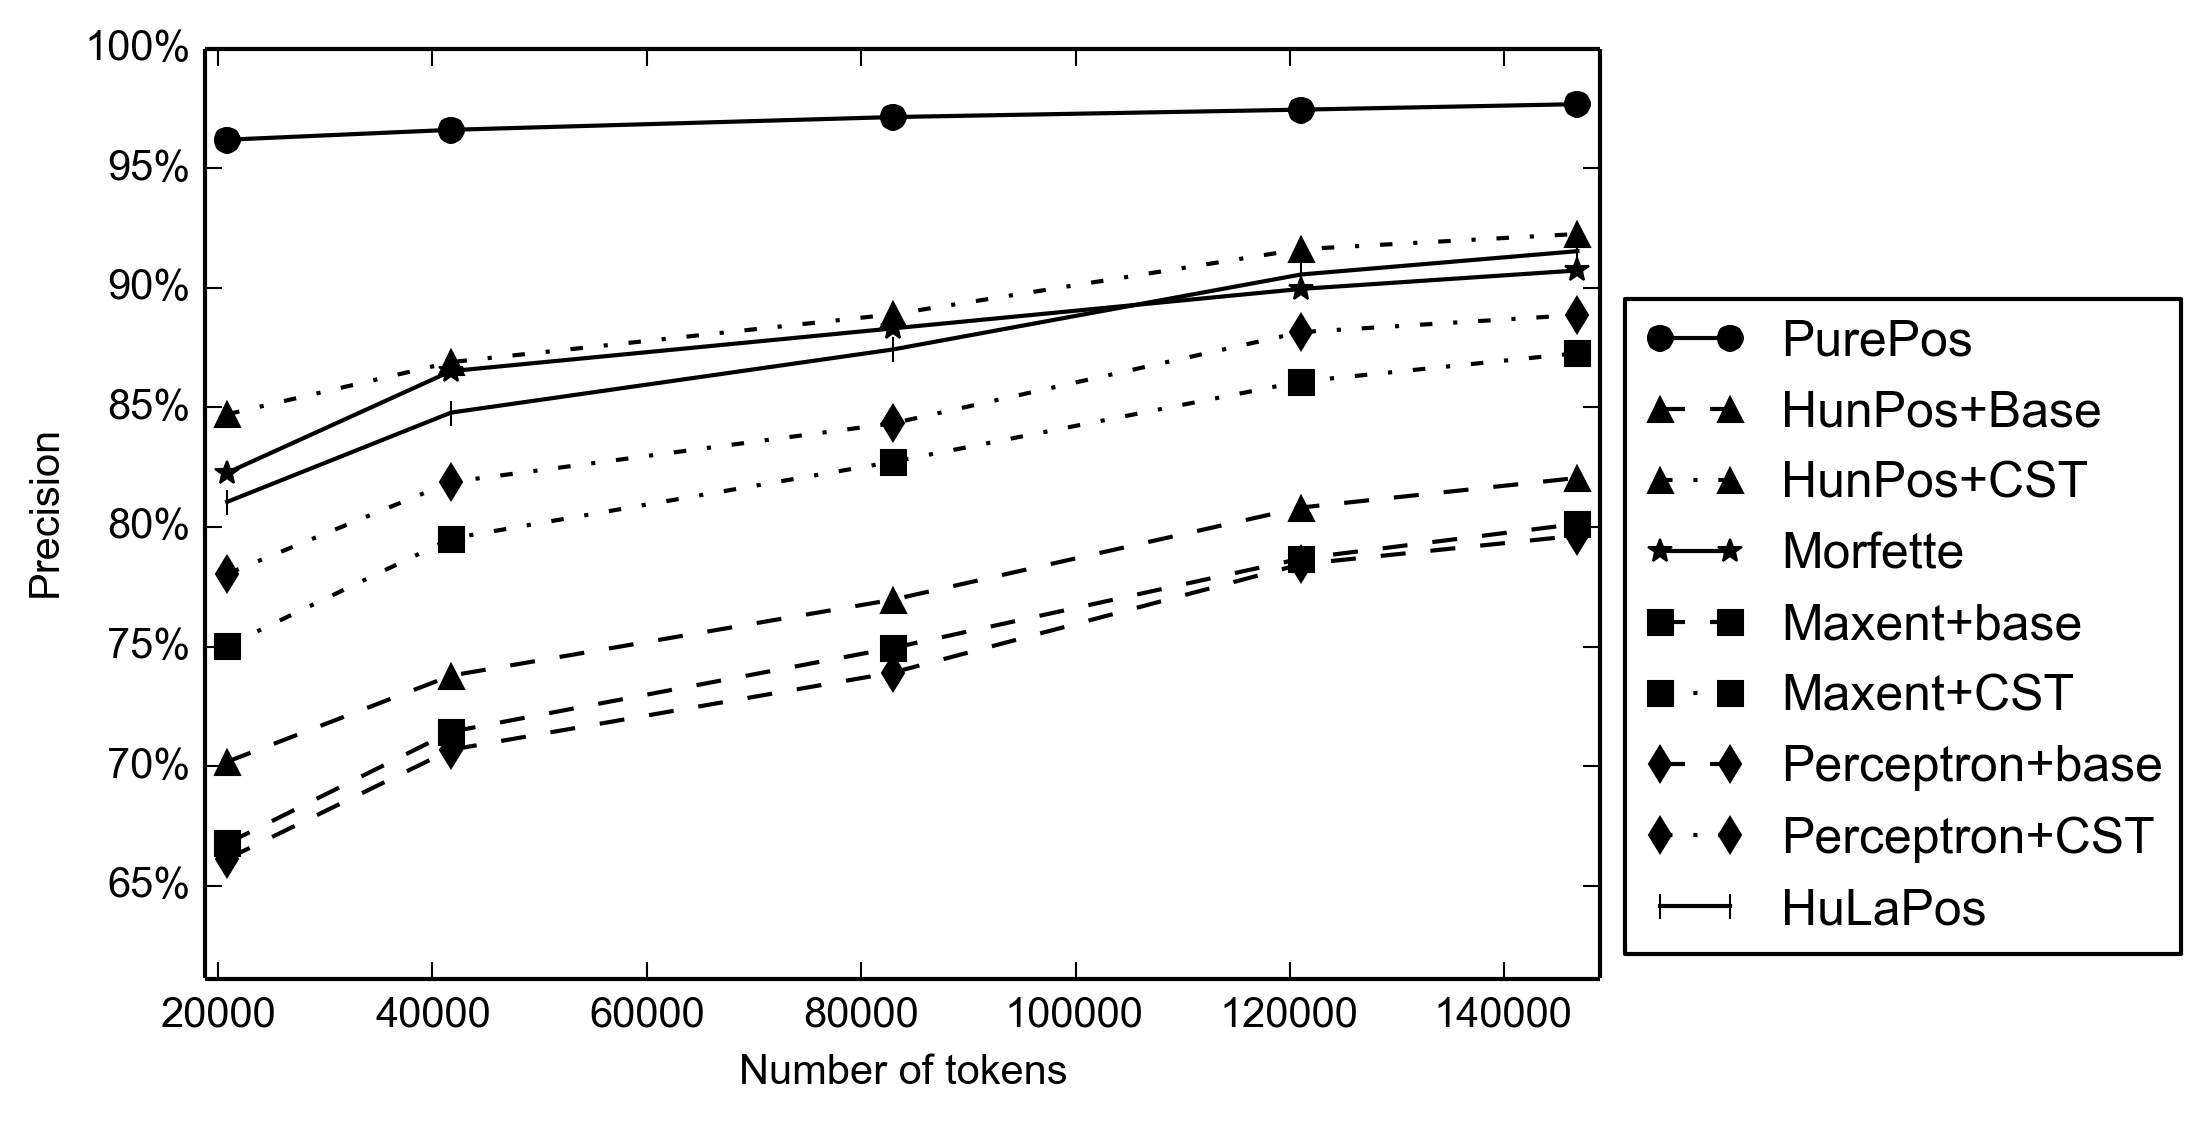
\includegraphics[width=1\textwidth]{MorphTagging/humor_token.png}
  \caption{Learning curves (regarding token accuracy) of full morphological taggers on the Szeged Corpus (using Humor labels)}
  \label{fig:humor-token}
\end{figure}

\begin{figure}[H]
  \centering
  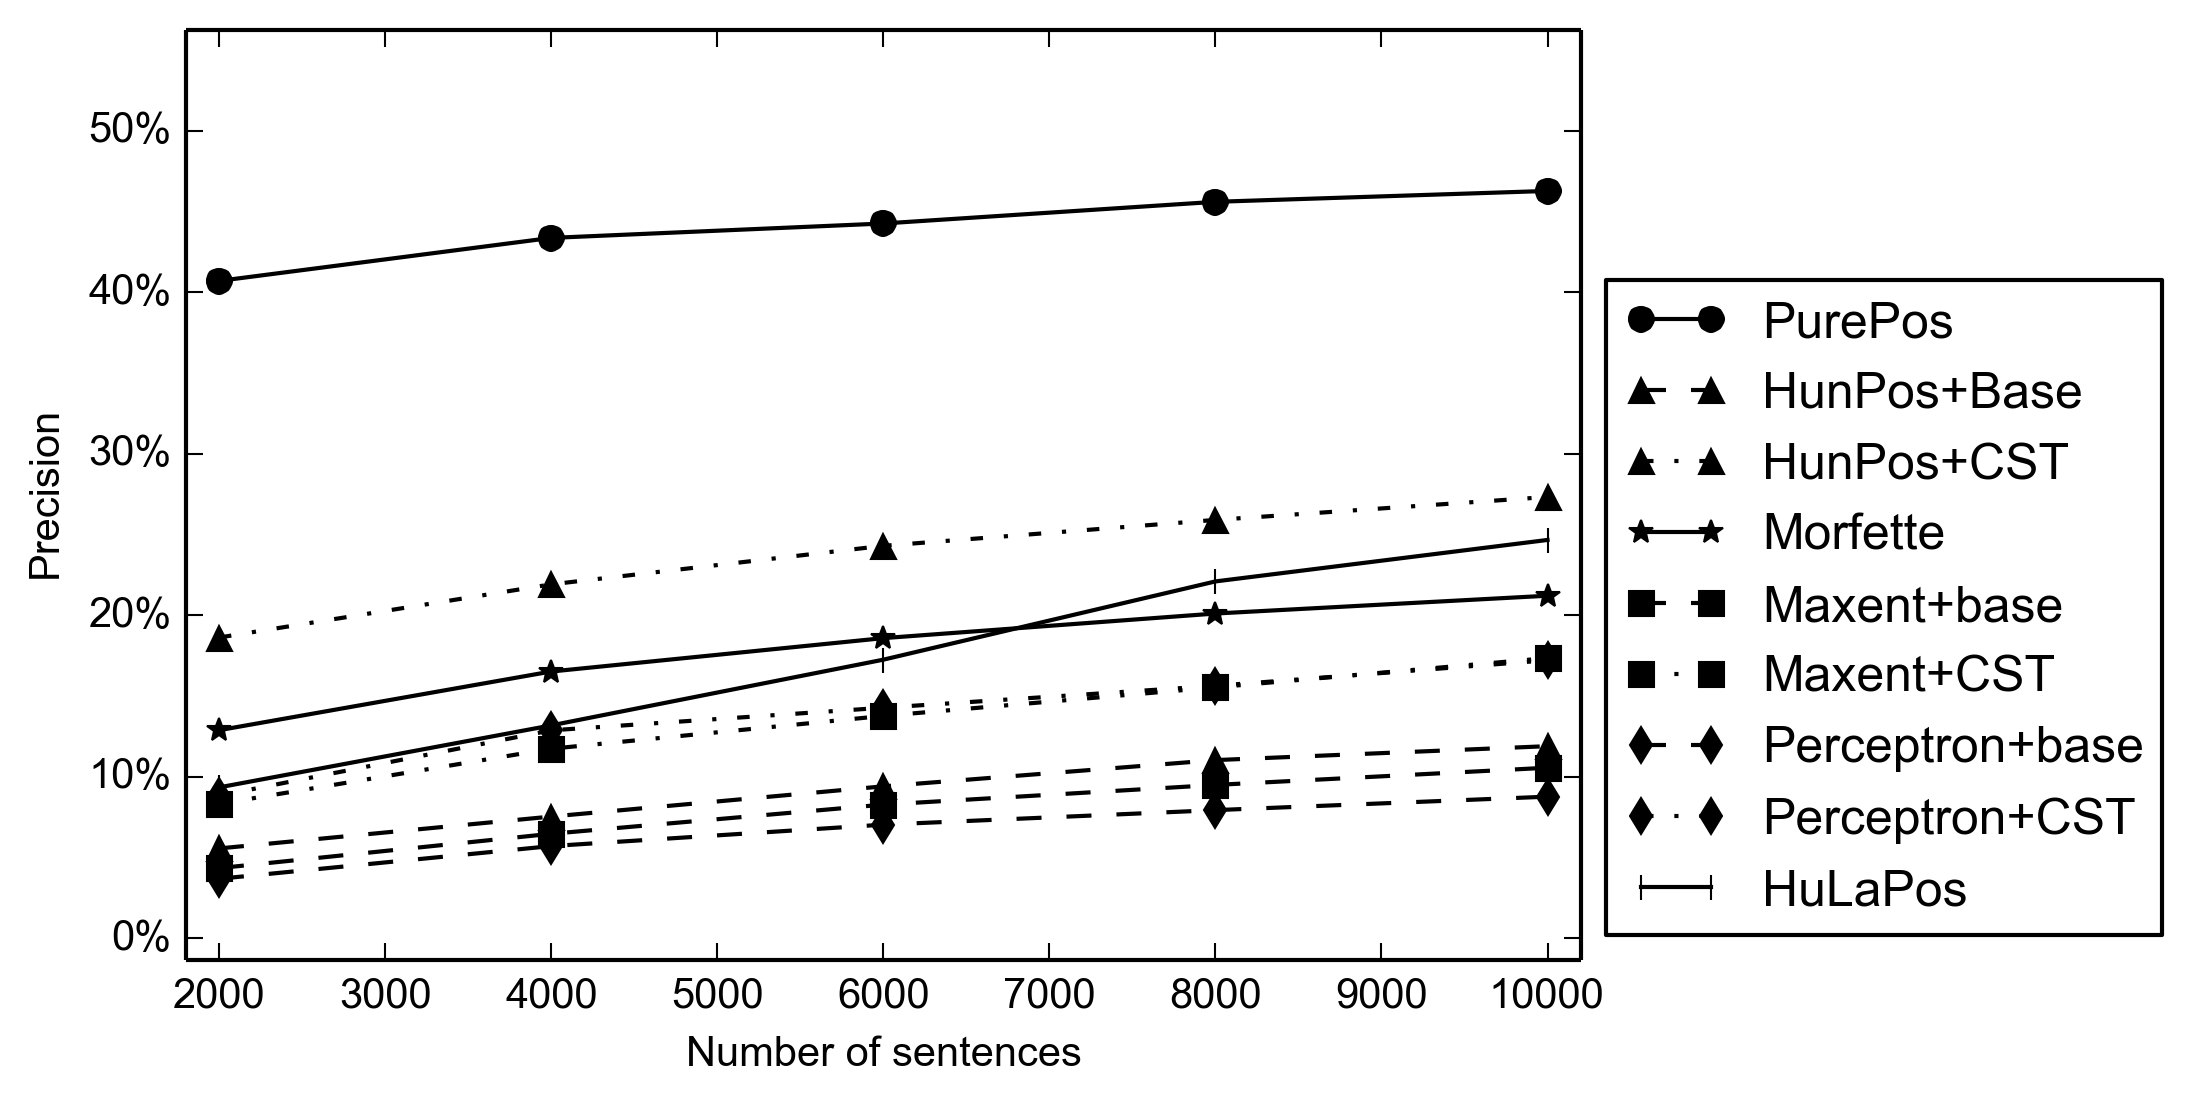
\includegraphics[width=1\textwidth]{MorphTagging/msd_sent.png} 
  \caption{Learning curves (regarding sentence accuracy) of full morphological taggers on the Szeged Corpus (using MSD labels)}
  \label{fig:msd-sent}
\end{figure}

\begin{figure}[H]
  \centering
  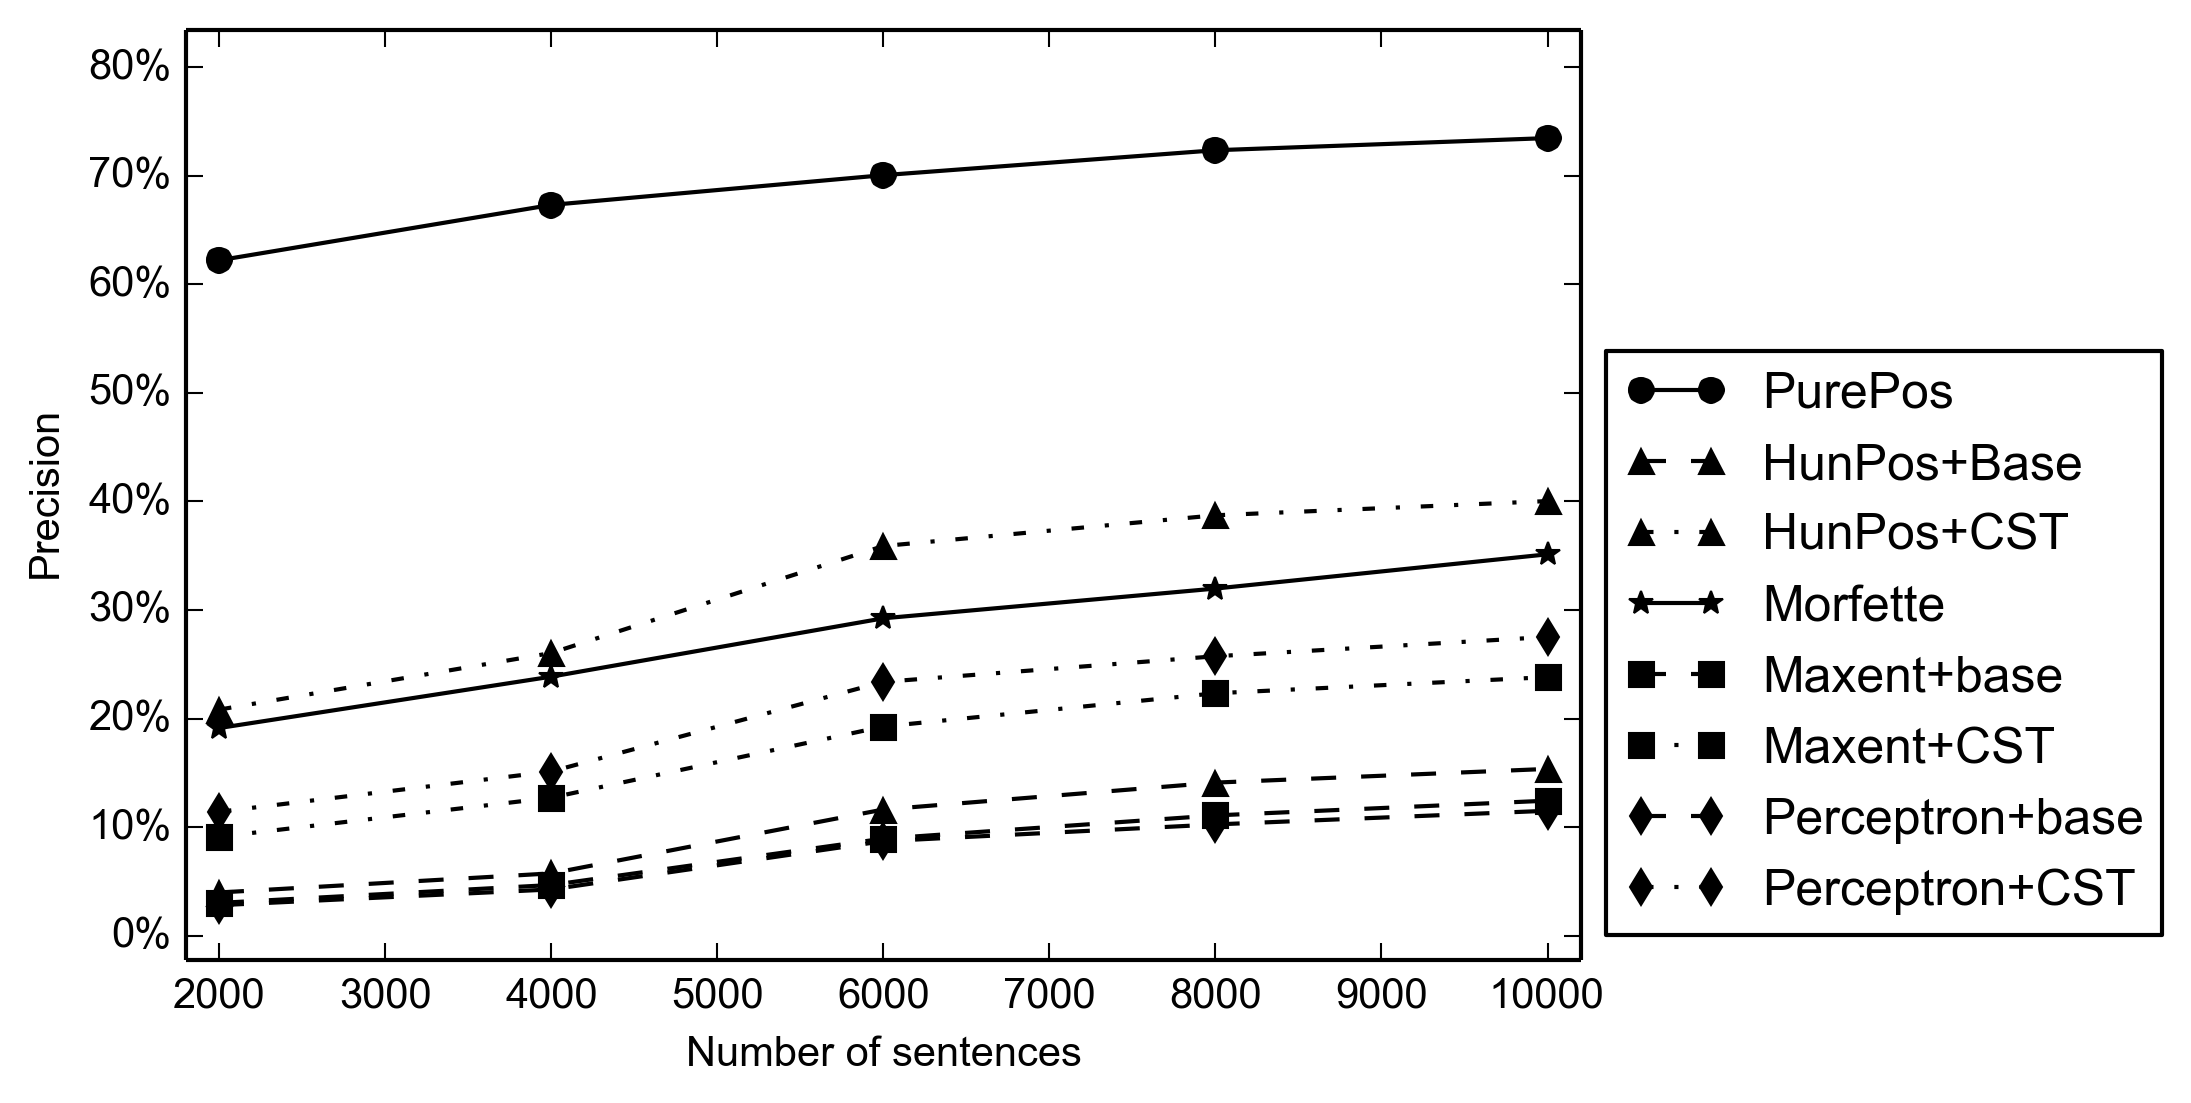
\includegraphics[width=1\textwidth]{MorphTagging/humor_sent.png}
  \caption{Learning curves (regarding sentence accuracy) of full morphological taggers on the Szeged Corpus (using Humor labels)}
  \label{fig:humor-sent}
\end{figure}

First, Figures \ref{fig:msd-token} and \ref{fig:humor-token} present morphological tagging accuracies of systems depending on the number of tokens in the training corpus. 
These results are in accordance with conclusions of our previous experiments; however, the differences revealed are higher. 
Further on, the large distance between the accuracy scores of PurePos and other tools confirms the effectiveness of our  hybrid approach in less-resourced scenarios.


Additionally, if we compare (cf. Figures \ref{fig:msd-sent} and \ref{fig:humor-sent}) the sentence-based accuracies of the taggers, the gap between their performance are much more emphasized. 
For example, having only 2,000 sentences for training (with MSD tags) the proposed algorithm results in 40.71\% sentence-level accuracy compared to the second best of 18.62\%.
The increased performance of our method is in a great part due to two things. 
On the one hand, the system presented extensively use  morphological analyzers, restricting the number of candidate analyses effectively thus providing more accurate analyses for \acrshort{oov} tokens.
On the other hand, Markov models are known to perform better in the case of resource-scare scenarios compared to discriminative methods.

In brief, we have shown that the architecture of PurePos allows producing accurate annotations when the amount of training data is limited. Therefore, our method could be used for morphological tagging scenarios when there is just a few thousand manually annotated sentences are available.

\subsubsection{The case of Middle- Old-Hungarian}
\label{sec:oldhungarian}

Next, we present a tagging task showing the effectiveness of all the hybrid components available in PurePos. 
In a project~\cite{NovakOMK,Novak2013} aiming at the creation of an annotated corpus of Middle Hungarian texts, an adapted version of the Hungarian Humor morphological analyzer \cite{NovakOMK} was used\footnote{The adaptation of Humor and the annotation were done by  Attila Novák and Nóra Wenszky. The author's contribution is the enhancement of the morphological tagging chain.}. 
This tool was originally made to annotate contemporary Hungarian, but the grammar and lexicon were modified to handle morphological constructions that existed in Middle Hungarian but have since disappeared from the language. 
In the experiments described here, we used a manually disambiguated portion of this corpus. The tokens were labeled using a rich variant of the Humor tag-set having cardinality over a thousand.

\begin{table}[H]
\centering
\caption{Number of clauses and tokens in the Old and Middle Hungarian corpus}\label{tab:oldhun-corpus}
\begin{tabular}{l r r r}
\hline
& Training & Development & Test \\
\hline
Documents & 140 & 20 & 30 \\
Clauses & 12,355 & 2,731 & 2,484 \\
Tokens & 59,926 & 12,656 &  11,763\\
\hline
\end{tabular}
\end{table}

The corpus was split into three parts (see Table \ref{tab:oldhun-corpus}) for the experiments. 
The tagger was trained on the biggest one, adaptation methods were developed on a separate development subcorpus, while final evaluation was done on the test set.
We used accuracy as an evaluation metric, but unambiguous punctuation tokens were \emph{not} taken into account (in contrast to how taggers are evaluated in general). 
They are ignored because the corpus contains a relatively large amount of punctuation marks which would distort the comparison.
Methods were evaluated in two ways: full morphological disambiguation accuracies were calculated for tokens and they were also computed to obtain clause-level accuracy values. 
In addition, \gls{err} \eqref{eq:err} is calculated measuring the percentage of mistakes ($E$) of a baseline tagger ($b$) that are corrected by an enhanced method ($n$). 

\begin{equation}\label{eq:err}
\err(b,n) = \frac{E(b)-E(n)}{E(b)}
\end{equation}

We used the improved trigram-based algorithm derived from HunPos and implemented in PurePos (PP) as a baseline \gls{pos} tagger. 
This basic chain is enhanced step-by-step investigating the impact of each component.
First, the \acrshort{ma} and the new lemmatization method is analyzed on the development set (cf. Table \ref{tab:oldhun-baselines}). 

\begin{table}[H]
\centering
\caption{Baseline disambiguation accuracies on the development set. BL is the baseline unigram lemmatizer, while CL is đthe proposed one. PPM and PP both denote the PurePos tagger, however the first uses a morphological analyzer.}\label{tab:oldhun-baselines}
\begin{tabular}{l r r r}
\hline
 & Tokens & Clauses \\
\hline
% PP+BL & 93.20\% & 88.99\% & 55.58\% \\
PP + BL  & 88.99\% & 55.58\% \\
% PP+SL & 93.20\% & 89.01\% & 51.78\% \\
% PPM+BL & 97.77\% & 97.22\% & 84.85\% \\
PPM + BL  & 97.22\% & 84.85\% \\
% PPM+SL & 97.77\% & 97.50\% & 85.98\% \\
PP + CL & 92.14\% & 65.40\% \\
PPM + CL & 97.58\% & 86.48\% \\
\hline
\end{tabular}
\end{table}


On the one hand, we compare the \gls{pos} tagging method of PurePos with (PPM) and without the morphological analyzer (PP).
On the other hand, the simple unigram-based (BL) lemmatizer (cf. Section \ref{sec:purepos-guesser}) is evaluated against the proposed one (CL). 
First, it was found that the usage of a morphological component is indispensable. 
Next, results show that the proposed algorithm yields a significant error rate reduction compared to the baseline. 
This improvement is even more notable  (28.42\% \acrshort{err}) when a dedicated morphological analyzer is not used.

Below, several experiments are presented to exhaust hybrid facilities of PurePos, thus yielding a more accurate tagger. 
To that end, the development set was utilized to analyze common error types and to develop hypotheses.

\paragraph{Mapping of tags}

In contrast to other Hungarian annotation projects, the tag-set of the historical corpus distinguishes verb forms that have a verbal prefix from those that do not, because this is a distinction important for researchers interested in syntax.\footnote{Hungarian verbal prefixes or particles behave similarly to separable verbal prefixes in most Germanic languages: they usually form a single orthographic word with the verb they modify, however, they are separated in certain syntactic constructions.} 
This practically doubles the number of verb tags\footnote{320 different verb tags occur in the corpus excluding verb prefix vs. no verb prefix distinction. This is just a fraction of the theoretically possible tags.}, which results in data sparseness problems for the tagger. 
In the case of a never encountered label having a verbal prefix marking, one can calculate probability estimates for that tag by mapping it to one without a verbal prefix. 
This solution is viable, since the distribution of prefixed and non-prefixed verbs largely overlap. 
Applying this enhancement (TM), we could increase the accuracy of the system on the development set (to 86.53\% clause level accuracy) notably.

\paragraph{Preprocessing}

Another point of improvement is to filter analyses of Humor (FI). 
Exploiting the development set, a preprocessing script was set up which has five simple rules. 
Three of them catches the tagging of frequent phrases such as \emph{az a} `that' in which \emph{az} must be a pronoun. 
Further on, two domain specific lexicons were employed to correct the erroneous annotation of proper names that coincide with frequent common nouns or adjectives. 
Using these correction rules the overall performance on the development set was further raised to 86.77\% clause accuracy.


%%%%%%%%%%%%%%%%%%%%%%%%%%%%%%%%%%%%%%%%%%%%%%%%%%%%%%%%%%%%%%%%%%%%

\paragraph{$k$-best output}
The $k$-best output of the tagger can either be used as a representation to apply upstream grammatical filters to or as candidates for alternative input to higher levels of processing. 
Five-best output for our test corpus has yielded an upper limit for attainable clause accuracy of 94.32\% (on the development set). 
%These can either be used as a representation to apply upstream grammatical filters to or as candidates for alternative input to higher levels of processing.
While it is not directly comparable with the ones above, this feature could e.g. be used by syntactic parsers.


\begin{table}[H]
\centering
\caption{Disambiguation accuracies of the hybrid tool on the test set. TM is the tag mapping approach, while FI denotes the rule-based preprocessing.}
\label{tab:oldhun-test}
\begin{tabular}{l r r r}
\hline
 & Token & Clauses  \\
\hline
Baseline  & 89.47\% & 55.07\% \\
PurePos  & 96.48\% & 80.95\% \\
\hspace{0.2cm} + TM  & 96.51\% & 81.17\% \\
\hspace{0.2cm} + FI  & 96.60\% & 81.55\% \\
\hspace{0.2cm} + all  & 96.63\% & 81.77\% \\
\hspace{0.2cm} + all with \emph{k}-best  & 98.66\% & 92.30\% \\
\hline
\end{tabular}
\end{table}
 
Enhancements are validated evaluating them on the test set.
Data in Table \ref{tab:oldhun-test} show that each linguistic component improves the overall chain significantly\footnote{We used the Wilcoxon matched-pairs signed-rank test at p < 0.05}.
Further on, using the $5$-best output sequence of the tagger one can further improve the accuracy of the tool.
Golden tags and lemmata are available for 92.30\% of the clauses and for 98.66\% of the tokens between the top five annotation sequence.

We have shown that one can further increase the tagging accuracy by employing hybrid facilities of PurePos. 
%In this section, linguistic knowledge has been used to raise the overall accuracy.
First, rules were employed filtering our erroneous analysis candidates, then unseen tags were mapped to previously seen ones successfully. 
Finally, we have shown that the 5-best output contains significantly more golden annotations.



